% Thesis discussion, beamer version.
% Build: latexmk -pdf thesis_presentation.tex
% Charts and backup tables are generated from the thesis tables: python3 ../src/make_assets.py
\documentclass[aspectratio=169,11pt]{beamer}

\usepackage[T1]{fontenc}
\usepackage[utf8]{inputenc}
\usepackage{lmodern}
\usefonttheme[onlymath]{serif}
\usepackage{amsmath,amssymb,bm}
\usepackage{booktabs,array}
\usepackage{tikz}
\usetikzlibrary{arrows.meta,positioning,calc}
\graphicspath{{figures/}{../../Latex/Figures/}}
% To rehearse with the speaker notes on a second screen, uncomment:
% \usepackage{pgfpages}\setbeameroption{show notes on second screen=right}

%%--- Title-slide data -------------------------------------------------------
\newcommand{\talktitle}{Imputation of Missing Data in Financial Time Series}
\newcommand{\talktitlelines}{Imputation of Missing Data\\in Financial Time Series}
\newcommand{\talksubtitle}{From reconstruction error to downstream decisions}
\newcommand{\talkauthor}{Michele Carlo Fanelli}
\newcommand{\talksupervisor}{Francesco Corielli}
\newcommand{\talkinstitute}{Bocconi University}
\newcommand{\talkyear}{2025/2026}
\hypersetup{pdftitle={\talktitle}, pdfauthor={\talkauthor}}

%%--- Palette (shared with the PowerPoint version) ---------------------------
\definecolor{ink}{HTML}{14213D}
\definecolor{accent}{HTML}{E4572E}
\definecolor{muted}{HTML}{6B7280}
\definecolor{tint}{HTML}{F2F4F7}
\definecolor{rulec}{HTML}{D0D5DD}
\definecolor{emc}{HTML}{FF9500}

%%--- Theme ------------------------------------------------------------------
\hyphenpenalty=10000
\exhyphenpenalty=10000
\setbeamertemplate{navigation symbols}{}
\setbeamercolor{normal text}{fg=ink!92!black,bg=white}
\setbeamercolor{structure}{fg=ink}
\setbeamercolor{frametitle}{fg=ink}
\setbeamercolor{block title}{fg=ink,bg=tint}
\setbeamercolor{block body}{fg=ink!92!black,bg=tint}
\setbeamertemplate{blocks}[rounded][shadow=false]
\setbeamerfont{frametitle}{size=\large,series=\bfseries}
\setbeamerfont{block title}{size=\small,series=\bfseries}
\setbeamertemplate{itemize item}{\raisebox{0.15ex}{\color{accent}\rule{0.55ex}{0.55ex}}}
\setbeamertemplate{itemize subitem}{\raisebox{0.2ex}{\color{muted}\rule{0.45ex}{0.45ex}}}
\setbeamertemplate{enumerate item}{\color{accent}\bfseries\insertenumlabel.}
\setbeamersize{text margin left=6mm,text margin right=6mm}
\setlength{\leftmargini}{1.1em}

\newif\ifbackup
\providecommand{\mainframecount}{12}
\makeatletter
\newcommand{\recordmainframes}{\write\@auxout{\string\gdef\string\mainframecount{\the\c@framenumber}}}
\makeatother

\newcommand{\navitem}[2]{%
  \ifnum\value{section}=#1{\color{ink}\bfseries #2}\else{\color{muted!65}#2}\fi}
\setbeamertemplate{headline}{%
  \vskip2.6mm%
  \hbox to \paperwidth{\hskip6mm%
    {\tiny\color{muted}\ifbackup Backup material\else\talktitle\fi}\hfill
    {\tiny\ifbackup\else\navitem{1}{Introduction}\hskip3.5mm\navitem{2}{Methodology}%
      \hskip3.5mm\navitem{3}{Results}\hskip3.5mm\navitem{4}{Conclusion}\fi}%
    \hskip6mm}}
\setbeamertemplate{frametitle}{%
  \vskip0.4mm\usebeamerfont{frametitle}\usebeamercolor[fg]{frametitle}\insertframetitle\par
  \vskip-0.6mm}
\setbeamertemplate{footline}{%
  \hbox to \paperwidth{\hskip6mm%
    
\begin{tikzpicture}[baseline=-0.25ex]
      \fill[ink!25] (0,0) rectangle ++(0.9mm,0.9mm);
      \fill[ink!25] (1.3mm,0) rectangle ++(0.9mm,0.9mm);
      \fill[accent] (2.6mm,0) rectangle ++(0.9mm,0.9mm);
    \end{tikzpicture}\hskip1.5mm%
    {\tiny\color{muted}\talkauthor\ \textperiodcentered\ \talkinstitute}\hfill
    {\tiny\color{muted}\ifbackup Backup \insertframenumber\else\insertframenumber\,/\,\mainframecount\fi}%
    \hskip6mm}\vskip2.4mm}

\newcommand{\src}[1]{{\par\vskip1mm\tiny\color{muted}#1\par}}
\newcommand{\kpi}[1]{{\color{accent}\bfseries #1}}
\newcolumntype{L}[1]{>{\raggedright\arraybackslash}p{#1}}
\newcolumntype{G}[1]{>{\raggedright\arraybackslash\leavevmode\color{muted}}p{#1}}

\begin{document}

%%==========================================================================
\begin{frame}[plain,t]
\note{Introduce the problem in one sentence: financial panels always have holes, and the way they are filled changes what any model built on them concludes. The talk follows the thesis: motivation, design, results, then the two downstream evaluations.}
\begin{tikzpicture}[remember picture,overlay]
  \begin{scope}[shift={($(current page.north east)+(-57mm,-27mm)$)}]
    \foreach \r in {0,...,9}{\foreach \c in {0,...,15}{
      \fill[ink!9] (\c*3.1mm,-\r*3.1mm) rectangle ++(2.5mm,2.5mm);}}
    \foreach \r/\c in {0/6,0/8,0/10,1/3,1/5,2/1,2/2,2/3,3/3,3/8,4/3,4/6,4/14,5/2,5/11,6/10,6/11,%
                       7/2,7/3,7/4,7/6,7/8,7/9,7/11,7/12,7/13,8/1,8/2,8/6,8/11,9/8,9/13}{
      \fill[accent] (\c*3.1mm,-\r*3.1mm) rectangle ++(2.5mm,2.5mm);}
  \end{scope}
\end{tikzpicture}
\vskip17mm
{\scriptsize\color{accent}\bfseries MASTER'S THESIS \textperiodcentered\ BOCCONI UNIVERSITY}\par
\vskip4mm
\begin{minipage}{0.62\textwidth}\raggedright
  {\LARGE\bfseries\color{ink}\talktitlelines\par}
  \vskip3.5mm
  {\normalsize\color{muted}\talksubtitle\par}
\end{minipage}
\vskip17mm
\begin{minipage}[t]{0.32\textwidth}
  {\tiny\color{muted}CANDIDATE}\par\vskip0.5mm
  {\small\bfseries\color{ink}\talkauthor}
\end{minipage}%
\begin{minipage}[t]{0.32\textwidth}
  {\tiny\color{muted}SUPERVISOR}\par\vskip0.5mm
  {\small\bfseries\color{ink}\talksupervisor}
\end{minipage}%
\begin{minipage}[t]{0.3\textwidth}
  {\tiny\color{muted}ACADEMIC YEAR}\par\vskip0.5mm
  {\small\bfseries\color{ink}\talkyear}
\end{minipage}
\end{frame}

%%==========================================================================
\section{Introduction}

\begin{frame}[t]{Financial data is never fully observed}
\note{Gaps are everywhere: order-book feeds drop quotes, trading halts, OTC bond tenors go unquoted for days, macro data arrive at mixed frequencies. The default fixes are not neutral: carrying the last price forward biases betas (Scholes and Williams, 1977), dropping incomplete dates is unbiased only under MCAR and loses much of the sample, a constant fill damps variances and correlations. Deep imputers assume MAR, usually implicitly through their masked training objective, and evaluation is almost always pointwise. Aim: score each imputation on its reconstruction accuracy and on the downstream model built on it, against the same model fitted on the complete panel. The four questions structure the results; each gets its answer at the end.}
\begin{columns}[T,onlytextwidth]
\begin{column}{0.38\textwidth}
{\tiny\color{muted}THE PROBLEM}\par\vskip2.5mm
\small\textbf{Gaps are everywhere}\par
{\scriptsize\color{muted}halts, dropped quotes, illiquid tenors}\par\vskip3mm
\textbf{The usual fixes distort risk}\par
{\scriptsize\color{muted}stale prices, lost dates, damped correlations}\par\vskip3mm
\textbf{Evaluation is pointwise}\par
{\scriptsize\color{muted}MAE or RMSE on the masked cells only}\par
\end{column}
\begin{column}{0.58\textwidth}
{\tiny\color{muted}RESEARCH QUESTIONS}\par\vskip2.5mm
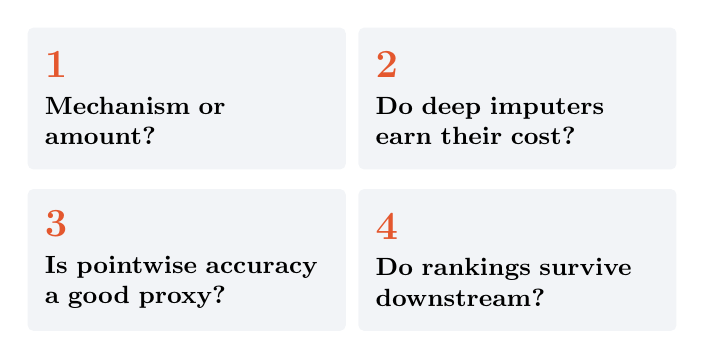
\begin{tikzpicture}[q/.style={rectangle, rounded corners=2pt, fill=tint, text width=36mm,
    minimum height=18mm, inner sep=2.2mm, anchor=north west, align=left, font=\small}]
  \node[q] at (0,0)        {{\color{accent}\Large\bfseries 1}\par\vskip0.8mm\textbf{Mechanism or amount?}};
  \node[q] at (42mm,0)     {{\color{accent}\Large\bfseries 2}\par\vskip0.8mm\textbf{Do deep imputers earn their cost?}};
  \node[q] at (0,-20.5mm)  {{\color{accent}\Large\bfseries 3}\par\vskip0.8mm\textbf{Is pointwise accuracy a good proxy?}};
  \node[q] at (42mm,-20.5mm) {{\color{accent}\Large\bfseries 4}\par\vskip0.8mm\textbf{Do rankings survive downstream?}};
\end{tikzpicture}
\end{column}
\end{columns}
\vfill
\begin{block}{}
\small\textbf{Aim.} Score each imputation on reconstruction \emph{and} on the model built on it, against an oracle fitted on the complete panel.
\end{block}
\vskip2mm
\end{frame}

%%==========================================================================
\section{Methodology}

\newcommand{\stagecontent}[5]{%
  \begin{minipage}[t][25mm][t]{29mm}\raggedright
  {\color{accent}\bfseries #1}\enspace\textbf{#2}\par\vskip0.8mm
  {\color{muted}#3}\par\vfill
  {\fontsize{17}{19}\selectfont\bfseries\color{ink}#4}\par\vskip0.6mm
  {\color{muted}#5}
  \end{minipage}}

\begin{frame}[t]{A controlled experiment on a complete equity panel}
\note{Start from a panel with no real missing data: S\&P 500 end-of-day prices from 1/1/2010 to 30/5/2026, stocks with any missing price removed, 50 sampled across industries. Delete entries under known rules, reconstruct, compare with the truth. Returns rather than prices because prices are positive, level dependent and non-stationary; a deleted return is a stylised missing price (a carried-forward price is a zero return, but the later catch-up return is not modelled). Every method may use the full sample, including dates after the gap: this is reconstruction after the fact, not real-time filling.}
\vskip3mm
\centering
\begin{tikzpicture}[node distance=4.6mm,
  stage/.style={rectangle, rounded corners=2pt, fill=tint, inner sep=2.2mm, font=\scriptsize},
  arr/.style={-{Stealth[length=2mm]}, ink!55, line width=0.9pt}]
  \node[stage] (a) {\stagecontent{1}{Complete panel}{50 S\&P~500 stocks, 2010 to 2026}{4125\,$\times$\,50}{daily log returns}};
  \node[stage, right=of a] (b) {\stagecontent{2}{Inject}{3 mechanisms $\times$ 5 levels}{15}{corrupted panels}};
  \node[stage, right=of b] (c) {\stagecontent{3}{Impute}{7 methods}{105}{imputed panels}};
  \node[stage, right=of c] (d) {\stagecontent{4}{Evaluate}{against the truth and an oracle}{7\,+\,2}{metrics, downstream models}};
  \foreach \u/\v in {a/b,b/c,c/d}{\draw[arr] (\u.east) -- (\v.west);}
\end{tikzpicture}
\vskip12mm
{\small\begin{tabular}{@{}c@{\hspace{9mm}}c@{\hspace{9mm}}c@{\hspace{9mm}}c@{\hspace{9mm}}c@{}}
\textbf{Daily log returns} & {\color{accent}\textbullet} & \textbf{Offline reconstruction} & {\color{accent}\textbullet} & \textbf{Known truth}\\[0.5mm]
{\scriptsize\color{muted}not prices} & & {\scriptsize\color{muted}the full sample is available} & & {\scriptsize\color{muted}for every deleted cell}
\end{tabular}\par}
\end{frame}

\begin{frame}[t]{Three mechanisms, matched on the share of missing cells}
\note{Sparse removes isolated cells, each independently with probability r. Gaps: n seed cells, each extended forward into a run of mean length ell trading days, within one asset. Stressed: dates at or above the p-quantile of the squared panel-average return lose each entry with probability h, other dates with r; so deletions line up across assets on the most volatile dates. The score is never shown to the imputer, which makes the pattern non-ignorable. Levels are matched on the expected share, so differences between patterns are due to the mechanism.}
\vskip-1.5mm
\centering
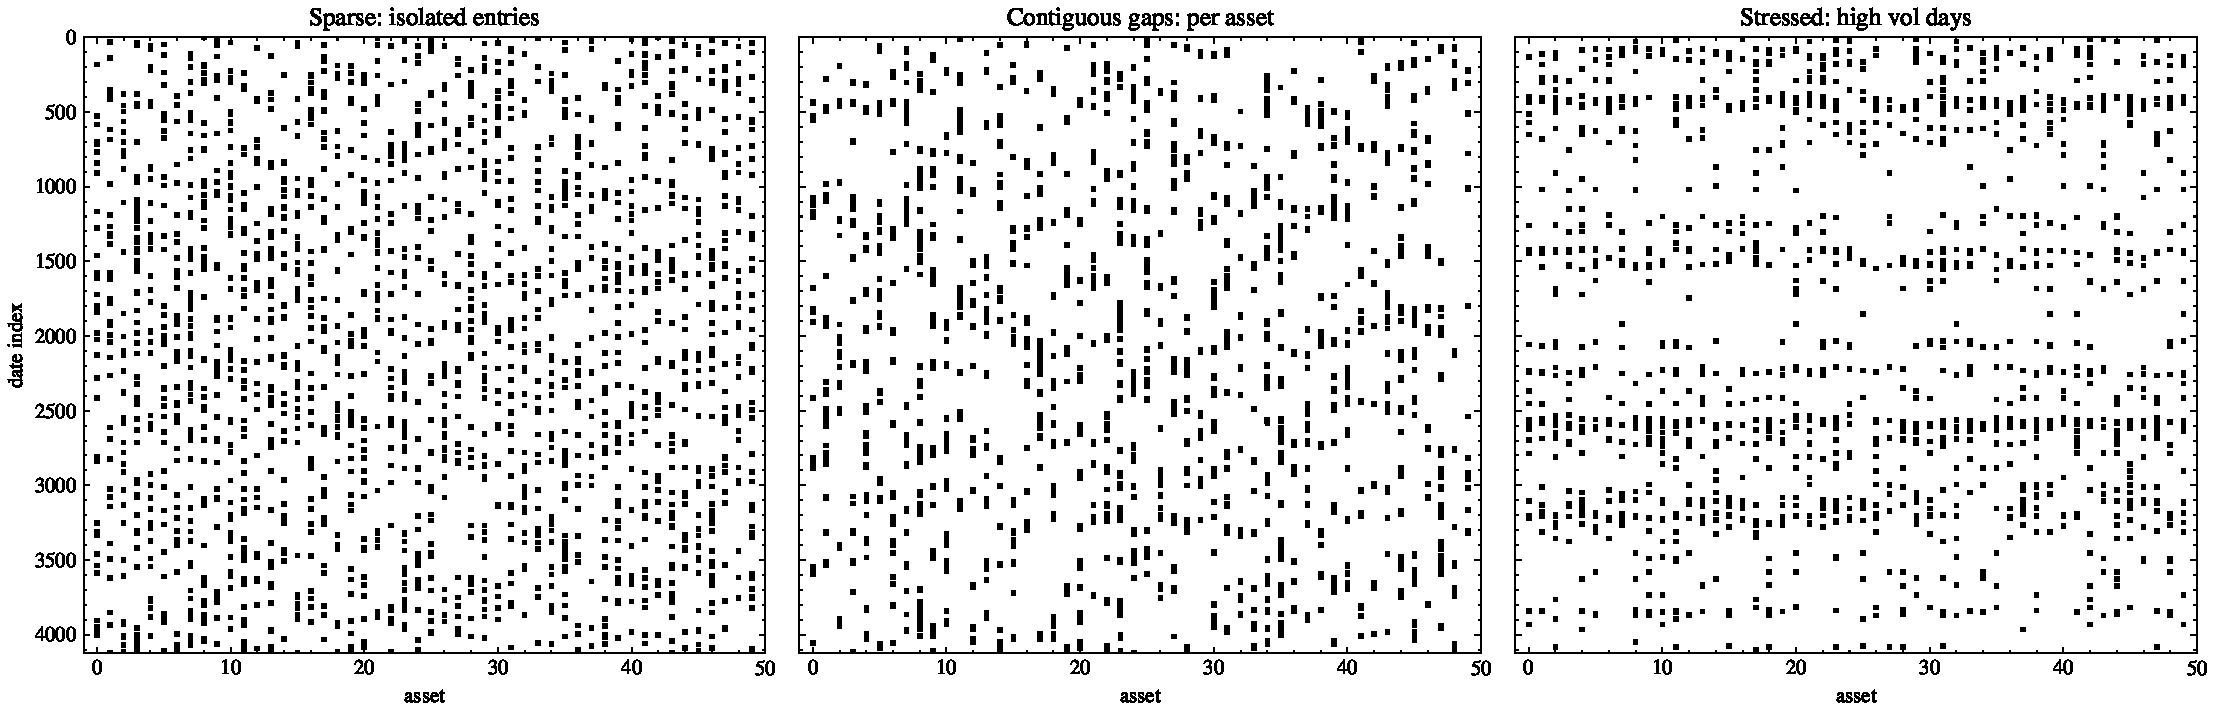
\includegraphics[width=0.68\textwidth]{missingness_examples.pdf}\par
\vskip1mm
{\small\begin{tabular}{@{}*{3}{>{\centering\arraybackslash}p{38mm}}@{}}
\textbf{Sparse} {\color{muted}MCAR}\newline{\scriptsize\color{muted}isolated cells} &
\textbf{Contiguous gaps} {\color{muted}MCAR}\newline{\scriptsize\color{muted}runs within one asset} &
\textbf{Stressed} {\color{accent}MNAR}\newline{\scriptsize\color{muted}the most volatile dates}
\end{tabular}\par}
\vskip2mm
{\centering\tiny\setlength{\tabcolsep}{6.5pt}
\begin{tabular}{@{}ll*{5}{c}@{}}
\toprule
\multicolumn{2}{@{}l}{Expected share of missing cells} & 0.1\% & 1\% & 5\% & 10\% & 30\% \\
\midrule
Sparse & $r$ & 0.001 & 0.01 & 0.05 & 0.1 & 0.3 \\
Gaps & $(n,\ell)$ & (20, 10) & (200, 10) & (1000, 10) & (1000, 20) & (2000, 30) \\
Stressed & $(r,h,p)$ & (0, 0.1, 0.99) & (0.005, 0.5, 0.99) & (0.04, 0.2, 0.95) & (0.05, 0.5, 0.9) & (0.2, 1, 0.9) \\
\bottomrule
\end{tabular}\par}
\end{frame}

\begin{frame}[t]{Seven methods, scored on the whole panel}
\note{Methods: Deletion drops every date with a missing value (Little and Rubin, 2019); Zero fills with 0, as if the price were carried forward; KNN is an inverse-distance average over the k nearest dates (Troyanskaya et al., 2001); Low-rank is iterative truncated SVD, a q-factor reconstruction (Mazumder et al., 2010); EM is Gaussian maximum likelihood with conditional-mean fill (Dempster et al., 1977); BRITS is a bidirectional RNN (Cao et al., 2018); CSDI is conditional score-based diffusion, median of 32 draws (Tashiro et al., 2021). EM is the one to watch: its fill is the conditional expectation given the other assets on the same date, the fill that minimises expected squared error. Metrics: pointwise ones look only at filled cells; the first five are invariant to permuting the dates, the temporal ones are not. Downstream: tangency portfolio w = Sigma^-1 mu / 1'Sigma^-1 mu, fitted on each panel, evaluated on the true returns, compared with the oracle (in sample); factor structure by variance shares and the subspace distance D_k between true and estimated leading eigenspaces.}
\begin{columns}[T,onlytextwidth]
\begin{column}{0.47\textwidth}
\vskip2mm
{\tiny\color{muted}SEVEN IMPUTERS}\par\vskip1.5mm
{\footnotesize\renewcommand{\arraystretch}{1.45}\setlength{\tabcolsep}{3pt}
\begin{tabular}{@{}G{19mm}L{47mm}@{}}
\toprule
Baselines & \textbf{Deletion}, \textbf{Zero} \\
Classical & \textbf{KNN}, \textbf{Low-rank}, {\color{emc}\textbf{EM}} \\
Deep learning & \textbf{BRITS} {\color{muted}(RNN)}, \textbf{CSDI} {\color{muted}(diffusion)} \\
\bottomrule
\end{tabular}\par}
\vskip5mm
\begin{block}{}
\centering
$\displaystyle \mathbb{E}\left[r_{t,m} \mid r_{t,o}\right] = \bm{\mu}_m + \bm{\Sigma}_{mo}\,\bm{\Sigma}_{oo}^{-1}\left(r_{t,o} - \bm{\mu}_o\right)$\\[1mm]
{\scriptsize\color{muted}EM fill: conditional mean given same-date observations}
\end{block}
\end{column}
\begin{column}{0.49\textwidth}
\vskip2mm
{\tiny\color{muted}SEVEN METRICS, TWO DOWNSTREAM MODELS}\par\vskip1.5mm
{\footnotesize\renewcommand{\arraystretch}{1.25}\setlength{\tabcolsep}{3pt}
\begin{tabular}{@{}G{25mm}L{45mm}@{}}
\toprule
Pointwise & MAE, RMSE \\
Marginal & VaRErr, WassErr \\
Second moment & CovErr \\
Temporal & AbsACFErr, LevErr \\
\midrule
Downstream & Tangency portfolio \\
 & Factor structure, $D_k$ \\
\bottomrule
\end{tabular}\par}
\end{column}
\end{columns}
\end{frame}

%%==========================================================================
\section{Results}

\begin{frame}[t]{Pointwise errors hit a floor at once, and EM sits on it}
\note{Daily returns are close to serially uncorrelated, so what can be known about a missing entry is carried by the other assets on the same date. EM's conditional mean extracts exactly that, so its MAE stays between 0.0071 and 0.0080 across all sparse levels. The five conditional methods are separated in the third decimal; the extra capacity of BRITS and CSDI has little to act on. The ranking is stable across patterns: EM is rarely beaten, and never by a wide margin.}
\begin{columns}[c,onlytextwidth]
\begin{column}{0.6\textwidth}
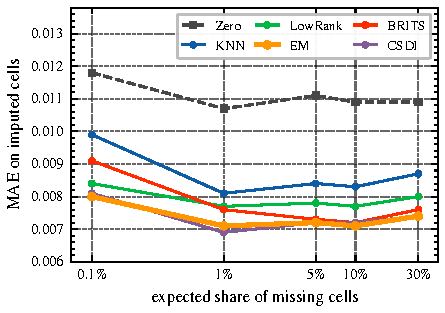
\includegraphics[width=\linewidth]{mae_floor.pdf}
\src{Sparse pattern, MAE on the imputed cells (Table 3.1).}
\end{column}
\begin{column}{0.36\textwidth}
{\tiny\color{muted}EM, MAE ACROSS SPARSE LEVELS}\par\vskip1mm
{\fontsize{20}{22}\selectfont\bfseries\color{emc}0.0071 to 0.0080}\par\vskip5mm
\small
\begin{itemize}\setlength{\itemsep}{2mm}
  \item Information is cross-sectional
  \item Conditional methods differ in the third decimal
  \item EM is rarely beaten
\end{itemize}
\end{column}
\end{columns}
\end{frame}

\begin{frame}[t]{Accurate cells do not make an accurate panel}
\note{MAE averages over the filled cells, so it stays flat; CovErr accumulates them over the panel, so it grows with the amount missing: EM's CovErr grows almost 40-fold while its MAE stays flat. Zero imputation shows the gap at its plainest: at sparse 0.3 its MAE is 1.5 times the best method's, its CovErr 8.9 times (ratios of Table 3.1 values). Even among good methods the families disagree: the best fill cell by cell is a conditional mean, less variable than the return it replaces; Low-rank loses to EM on MAE but beats it on CovErr at two stressed levels.}
\begin{columns}[T,onlytextwidth]
\begin{column}{0.49\textwidth}
\centering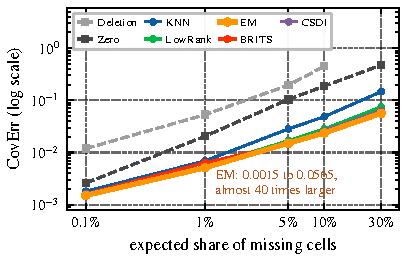
\includegraphics[width=\linewidth]{coverr_growth.pdf}
\end{column}
\begin{column}{0.49\textwidth}
\centering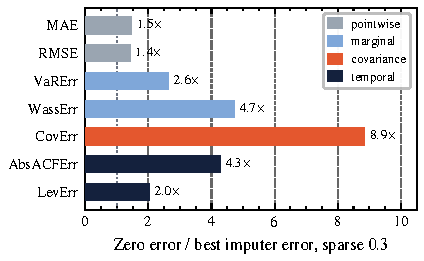
\includegraphics[width=\linewidth]{zero_ratio.pdf}
\end{column}
\end{columns}
\vskip2mm
\begin{columns}[T,onlytextwidth]
\begin{column}{0.315\textwidth}\centering
{\Large\bfseries\color{ink}almost 40$\times$}\par\vskip0.5mm
{\scriptsize\color{muted}growth of EM's CovErr, MAE flat}
\end{column}
\begin{column}{0.315\textwidth}\centering
{\Large\bfseries\color{ink}1.5$\times$}\par\vskip0.5mm
{\scriptsize\color{muted}Zero's MAE vs the best, sparse 0.3}
\end{column}
\begin{column}{0.315\textwidth}\centering
{\Large\bfseries\color{accent}8.9$\times$}\par\vskip0.5mm
{\scriptsize\color{muted}Zero's CovErr vs the best, sparse 0.3}
\end{column}
\end{columns}
\end{frame}

\begin{frame}[t]{The mechanism matters more than the amount}
\note{Read across at matched shares. Sparse and gaps are almost the same: with 49 other assets observed on each date, breaking the time axis costs a cross-sectional imputer little. The stressed pattern removes exactly those dates, aligned across assets, and the returns it removes are the largest ones, so the error sits in the target and no model capacity fixes it. BRITS falls behind where deletions are most extreme: MAE 0.0301 against EM's 0.0133 at (0, 0.1, 0.99). At (0.2, 1, 0.9) the ranking compresses: CovErr between 0.648 and 0.663 for every surviving model.}
\begin{columns}[c,onlytextwidth]
\begin{column}{0.56\textwidth}
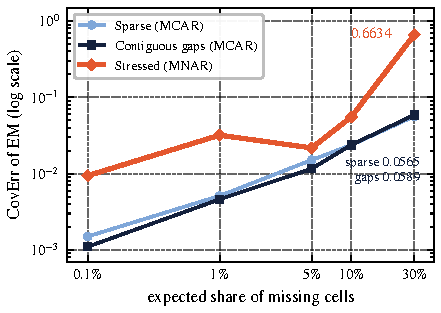
\includegraphics[width=\linewidth]{mechanism.pdf}
\src{EM, covariance error by pattern at matched shares (Tables 3.1 to 3.3).}
\end{column}
\begin{column}{0.4\textwidth}
{\footnotesize
\begin{tabular}{@{}lccc@{}}
\toprule
EM CovErr & Sparse & Gaps & Stressed \\
\midrule
10\% missing & 0.0237 & 0.0238 & 0.0554 \\
30\% missing & 0.0565 & 0.0589 & \kpi{0.6634} \\
\bottomrule
\end{tabular}\par}
\vskip5mm
\small
\begin{itemize}\setlength{\itemsep}{2mm}
  \item MCAR patterns: interchangeable
  \item Stressed MNAR removes the conditioning set
  \item At the heaviest level no method separates
\end{itemize}
\end{column}
\end{columns}
\end{frame}

\newcommand{\figtile}[3]{%
  \begin{column}{0.235\textwidth}\centering
  {\tiny\color{muted}#1}\par\vskip0.6mm
  {\large\bfseries\color{#3}#2}
  \end{column}}

\begin{frame}[t]{Downstream I: the portfolio amplifies the distortion}
\note{The tangency portfolio inverts the covariance, so small distortions turn into large positions. Oracle on the complete panel, annualised: mean 0.361, variance 0.049, Sharpe 1.636. Under heavy MCAR the variance rises from 0.049 to as much as 0.29 and L1 weight distances reach 14: the inverted covariance over-leverages. Under heavy MNAR the imputers never see the volatility; their portfolios end at little more than half of the oracle's cumulative return. EM and Low-rank are never the worst; BRITS has Sharpe 1.30 against EM's 1.51 at (0.05, 0.5, 0.9). Deletion: Sharpe near zero at sparse 0.1, singular covariance at the heavy levels. This is an in-sample diagnostic of fidelity, not a performance claim.}
\vskip-1.5mm
\centering
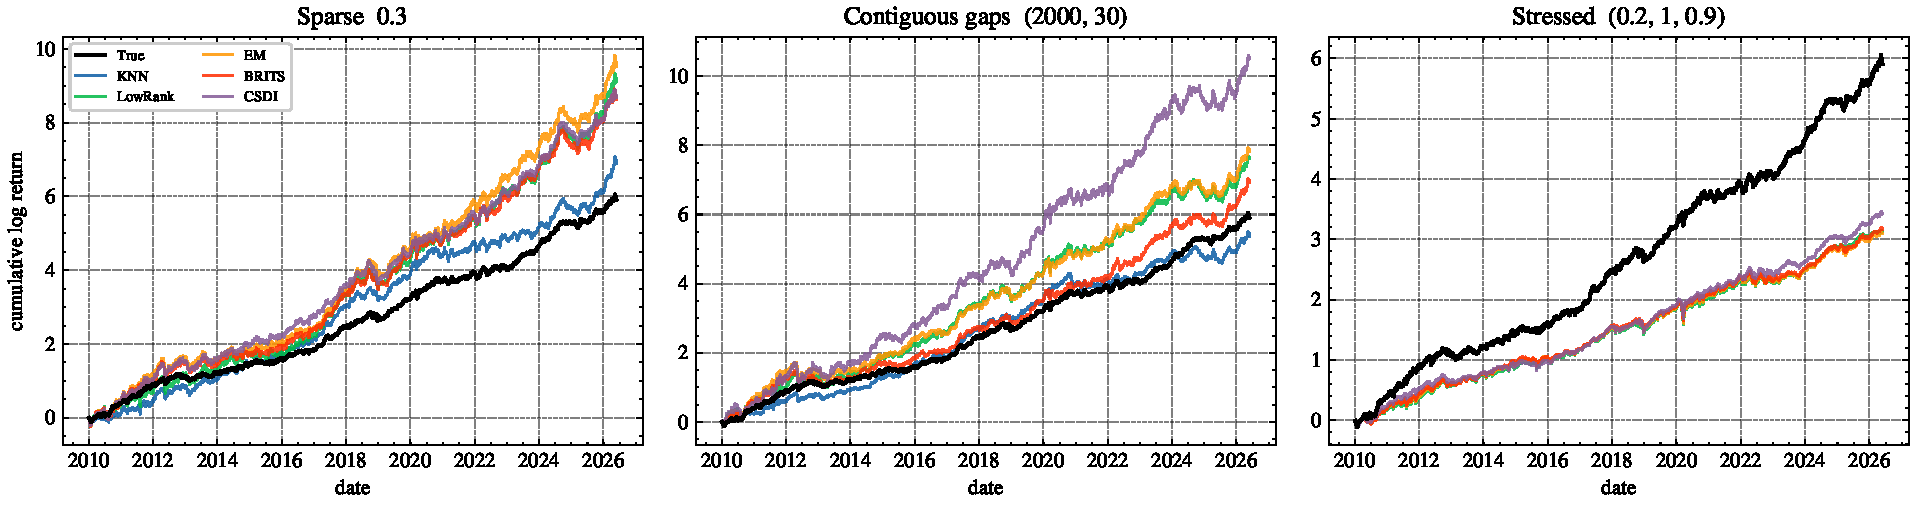
\includegraphics[width=\textwidth]{portfolio_realizations.pdf}\par
\vskip4mm
\begin{columns}[T,onlytextwidth]
\figtile{ORACLE SHARPE}{1.636}{ink}
\figtile{HEAVY MCAR: VARIANCE}{0.049 $\to$ 0.29}{accent}
\figtile{HEAVY MNAR: CUM.\ RETURN}{just over half}{accent}
\figtile{SHARPE, BRITS VS EM}{1.30 vs 1.51}{ink}
\end{columns}
\vskip3mm
\src{\centering In-sample diagnostic of reconstruction fidelity, not investment performance.}
\end{frame}

\begin{frame}[t]{Downstream II: a robust market factor, a fragile subspace}
\note{The first principal component is almost indestructible: D1 below 0.026 at sparse 0.3, under 1.5 degrees. The five-factor subspace is not: D5 from 0.14 to 0.39, six to eighteen times larger. Point imputations make the panel look more like its own factor model: conditional fills inflate the first factor's share from 41.74\% to between 45.6\% and 48.5\% at sparse 0.3. Low-rank has the largest D5 at 10 of 15 levels, although it imposes a factor structure. At (0.2, 1, 0.9) the first factor falls to about 25\% for all four methods that can be evaluated. Link to the portfolio: the inverse covariance loads most on the trailing directions, the ones recovered worst; the portfolio's error maximisation is the factor distortion seen through an inverse.}
\begin{columns}[T,onlytextwidth]
\begin{column}{0.64\textwidth}
\vskip1mm
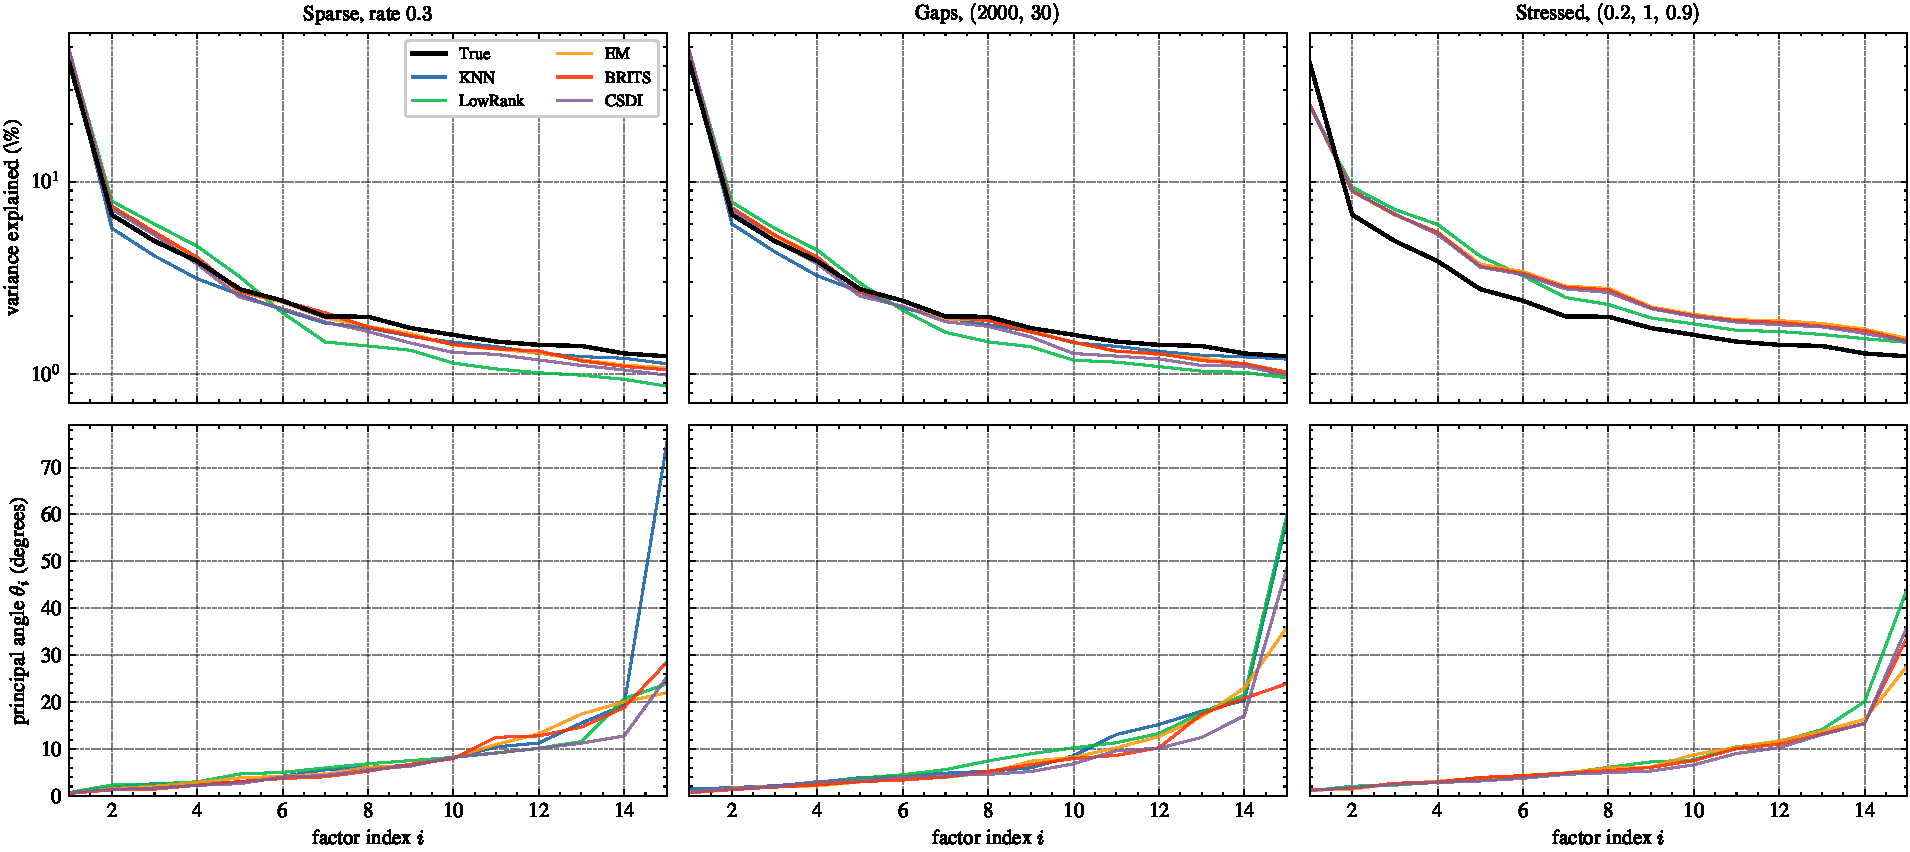
\includegraphics[width=\linewidth]{factor_structure.pdf}
\src{Variance shares (top) and principal angles (bottom), heaviest level of each pattern.}
\end{column}
\begin{column}{0.335\textwidth}
\vskip4mm
\renewcommand{\arraystretch}{1.5}\setlength{\tabcolsep}{2pt}
{\scriptsize
\begin{tabular}{@{}L{25mm}r@{}}
\toprule
Market factor, $D_1$ & $<$\,0.026 \\
Five factors, $D_5$ & \kpi{0.14 to 0.39} \\
PC1 share, true & 41.7\% \\
PC1 share, imputed & 45.6 to 48.5\% \\
Low-rank worst $D_5$ & 10 of 15 \\
\bottomrule
\end{tabular}\par}
\vskip3mm
\begin{block}{}
\centering\scriptsize
$\hat{\bm\Sigma}^{-1} = \sum_i \hat\lambda_i^{-1}\,\hat v_i \hat v_i^\top$\\[0.5mm]
{\color{muted}portfolio weight sits on the\\worst-recovered directions}
\end{block}
\end{column}
\end{columns}
\end{frame}

\newcommand{\costtile}[4]{%
  \begin{minipage}[t][24mm][t]{30mm}\centering
  {\fontsize{26}{28}\selectfont\bfseries\color{#2}#1}\par\vskip2.5mm
  {\scriptsize\bfseries #3\par\vskip0.8mm\mdseries\color{muted}#4\par}
  \end{minipage}}

\begin{frame}[t]{The deep models did not earn their cost}
\note{All of this ran on a single Apple Mac mini (M4, 16 GB), CPU-only PyTorch, with small networks (about 1.2e5 parameters for BRITS, 4.7e4 for CSDI), so the costs come from the algorithms. EM needs about a second to fill a 4125 x 50 panel. BRITS: just under an hour of training per panel (1e4 epochs). CSDI: just under four hours of training per panel, then about 24 minutes of sampling. Roughly seventy hours of neural training for the 15 levels, four fifths of it on CSDI. CSDI matches EM's accuracy at about four orders of magnitude more computation, and BRITS falls behind at two stressed levels.}
\vskip11mm
\centering
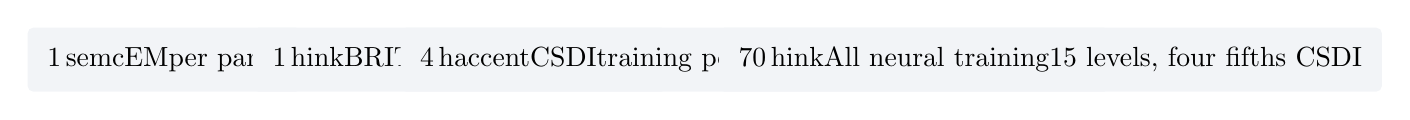
\begin{tikzpicture}[tile/.style={rectangle, rounded corners=2pt, fill=tint, inner sep=2.5mm, anchor=north}]
  \node[tile] at (0,0) {\costtile{1\,s}{emc}{EM}{per panel}};
  \node[tile] at (37.5mm,0) {\costtile{1\,h}{ink}{BRITS}{training per panel}};
  \node[tile] at (75mm,0) {\costtile{4\,h}{accent}{CSDI}{training per panel, plus 24 min sampling}};
  \node[tile] at (112.5mm,0) {\costtile{70\,h}{ink}{All neural training}{15 levels, four fifths CSDI}};
\end{tikzpicture}
\vskip9mm
{\large CSDI matches EM at about \kpi{four orders of magnitude} more computation}\par
\src{\centering Single Mac mini (M4, 16\,GB), CPU only. Approximate times, Section 3.3.}
\end{frame}

%%==========================================================================
\section{Conclusion}

\newcommand{\answer}[3]{%
  \node[rectangle, rounded corners=2pt, fill=tint, text width=67mm, minimum height=13mm,
        inner sep=2.2mm, anchor=north west, align=left] at (#1) {%
    {\color{accent}\bfseries\large #2}\enspace{\small #3}};}

\begin{frame}[t]{Conclusions}
\note{Go back to the four questions. 1: the mechanism, in this experiment; under MCAR the methods hold with 30\% missing, under stressed MNAR they break at far smaller shares, and at the heaviest level no method separates. 2: not here; EM is rarely beaten, CSDI matches it at four orders of magnitude more cost, BRITS falls behind at two stressed levels. 3: poor; Zero's MAE is 1.5 times the best and its CovErr about 9 times; conditional fills inflate the first factor from 41.7\% to as much as 48.5\%, which no pointwise metric registers. 4: largely, and the exceptions are informative; Low-rank has accurate cells but the worst five-factor subspace at 10 of 15 levels; Deletion is inefficient in the tables and gives unstable portfolios downstream. Limitations: one panel of fifty liquid large caps, daily, one run per configuration; injected missingness, the stressed pattern is a stylised MNAR; Gaussian EM without the Student-t refinement; both downstream models read the covariance; the portfolio is in sample; offline setting. Future work: causal imputation using only the past, downstream tests beyond the second moment (VaR backtests, hedging, trading rules), multiple imputation using the spread of the CSDI draws, larger cross sections and real gaps.}
\recordmainframes
\vskip1mm
\begin{tikzpicture}
  \answer{0,0}{1}{\textbf{The mechanism}, not the amount}
  \answer{73mm,0}{2}{Deep models: \textbf{no gain}, far higher cost}
  \answer{0,-15mm}{3}{Pointwise accuracy is a \textbf{poor proxy}}
  \answer{73mm,-15mm}{4}{Rankings \textbf{largely survive} downstream}
\end{tikzpicture}
\vskip3mm
\begin{block}{}
\centering\normalsize\textbf{Score an imputation against the use it is put to.}
\end{block}
\vskip2mm
{\scriptsize
\textbf{Limitations}\enspace{\color{muted}one panel, injected missingness, Gaussian EM, in-sample portfolio, offline}\par\vskip1mm
\textbf{Next}\enspace{\color{muted}causal imputation, multiple imputation, tests beyond the second moment}\par}
\vfill
\centering{\Large\bfseries\color{ink}Thank you}\par
\vskip2mm
\end{frame}


%%==========================================================================
\appendix
\backuptrue
\newcommand{\backupframe}[2]{%
  \begin{frame}[plain]{}
  \vskip2mm
  {\footnotesize\bfseries\color{ink}#1}\par\vskip1mm
  \input{backup/#2}
  \end{frame}}

\backupframe{Backup: evaluation scores under sparse missingness (Table 3.1; best value per level in bold)}{metrics_sparse}
\backupframe{Backup: evaluation scores under contiguous-gap missingness (Table 3.2; best value per level in bold)}{metrics_gaps}
\backupframe{Backup: evaluation scores under stressed missingness (Table 3.3; best value per level in bold)}{metrics_stressed}
\backupframe{Backup: optimal portfolio at every level (Tables 3.4 to 3.6; best Sharpe in bold)}{portfolio}
\backupframe{Backup: factor structure at every level (Tables 3.7 to 3.9; best $D_5$ in bold)}{factors}

\end{document}
